\selectlanguage{italian}

Il Modello Standard è una teoria incompleta, in quanto non riesce a spiegare, ad esempio, i valori delle masse delle particelle, le quali rimangono dei parametri liberi del modello, oltre a non includere affatto la gravità.

\section{Materia oscura}

Le osservazioni astronomiche indicano che la materia barionica costituisce soltanto il 4\% della materia totale nell'Universo: il restante 96\% è diviso tra materia oscura (22\%) ed energia oscura (74\%).

\subsection{Evidenze sperimentali}

Le prime evidenze dell'esistenza della materia oscura si ebbero negli anni 1930s, quando Zwicky e Smith osservarono le velocità delle galassie all'interno di clusters e si resero conto che queste erano $ 10-100 $ volte maggiori a quelle calcolate dalla massa visibile, in particolare ai bordi dei clusters, suggerendo l'esistenza di ulteriore massa per spiegare l'eccessiva forza gravitazionale; questa, però, non era un'evidenza abbastanza convincente, in quanto misure di questo tipo erano prone ad errori sistematici dovuti alla difficoltà di distinguere le galassie interne al cluster da quelle esterne e da quelle sullo sfondo.\\
Si ricordi che un sistema many-body gravitazionalmente legato ubbidisce al \textit{teorema del viriale}:
\begin{equation}
	2 \braket{K} = - \braket{U_g}
	\quad \Rightarrow \quad
	\braket{v^2} \approx G M \braket{r^{-1}}
	\label{eq:11.1}
\end{equation}
Inoltre, la velocità di una galassia rispetto alla Terra può essere misurata dal Doppler shift delle sia linee spettrali atomiche, note dalle misure in laboratorio:
\begin{equation}
	z \defeq \frac{\lambda_{\text{observed}} - \lambda_{\text{emitted}}}{\lambda_{\text{emitted}}} = \sqrt{\frac{1 + v/c}{1 - v/c}} - 1 \approx \frac{v}{c}
	\label{eq:11.2}
\end{equation}
dove l'approssimazione è valida per velocità non-relativistiche $ v \ll c $. L'effetto Doppler genera un blueshift $ z < 0 $ per oggetti che si avvicinano ed un redshift $ z > 0 $ per oggetti che si allontanano.\\
Evidenze empiriche più solide dell'esistenza della materia oscura si ebbero negli anni 1970s, quando Vera Rubin e Ken Freeman osservarono le rotation curves di varie galassie e notarono che le velocità delle stelle ai bordi delle galassie non potevano essere spiegate dalla sola materia osservata: l'andamento funzionale previsto dal modello Kepleriano è $ v^2 = \frac{GM}{r} $ ($ F_c = F_g $), ma ciò non è quello che si evince dai dati osservati, i quali invece riportano delle rotation curve essenzialmente piatte. L'unica spiegazione possibile, senza modificare la teoria della gravità, è che ciascuna galassia sia avvolta da un dark matter halo molto più esteso della galassia stessa e 10 volte più massivo.

\subsubsection{Gravitational lensing}

Il gravitational lensing è un fenomeno previsto dalla Relatività Generale ed è causato dalla deformazione della luce proveniente da una sorgente lontana ad opera un oggetto massimo lungo il suo percorso: infatti, analogamente alla deflessione di corpi massivi, anche la luce viene deviata dalla presenza di campi gravitazionali. Il gravitational lensing, dunque, può essere utilizzato per studiare la distribuzione di massa dell'oggetto che causa la deflessione della luce.\\
Un caso particolare di gravitational lensing è l'\textit{Einstein ring}, fenomeno che avviene col perfetto allineamento di sorgente, deflettore e Terra: l'immagine distorta della sorgente prenderà la forma di un anello attorno al corpo massivo che causa il lensing. In particolare, c'è una relazione tra la massa $ M $ di tale corpo massivo e la dimensione angolare $ \theta $ (in radianti) dell'Einstein ring:
\begin{equation}
	\theta = \sqrt{\frac{4GM}{c^2} \frac{D_{LS}}{D_S D_L}}
	\label{eq:11.3}
\end{equation}
dove $ D_L $, $ D_S $ e $ D_{SL} $ sono le angular diameter distances\footnote{distanza definita a partire dalla dimensione fisica $ x $ di un oggetto e dalla sua dimensione angolare $ \theta $ come $ d = \frac{x}{\theta} $.} rispettivamente tra Terra e lente, tra Terra e sorgente e tra lente e sorgente.\\
A partire da questo fenomeno, nel 1937 Zwicky ipotizzò la possibilità di misurare la distribuzione di materia oscura in un galaxy cluster tramite lo studio delle galassie in background che subiscono lensing dal cluster stesso: questo metodo d'osservazione è stato realizzato per la prima volta a metà anni 1990s. Anche studiando le collisioni tra galaxy clusters si è trovato che il centro di massa misurato dal gravitational lensing non corrisponde a quello misurato per la materia visibile, andando a confermare l'ipotesi dell'esistenza della materia oscura.

\subsection{Ipotesi teoriche}

Tutte i dati sperimentali finora rilevati sulla materia oscura sono di natura gravitazionale, dunque non delineano la sua natura a livello particellare: in particolare, questi dati sono fittati consistentemente da modelli che prevedono costituenti di materia oscura con masse da $ 10^{-22} \ev/c^2 $ a $ 100 M_\odot $.\\
Negli anni, si sono susseguiti e si susseguono numerosi esperimenti per sondare questi 80 ordini di grandezza, e molte ipotesi sono state ruled out: un esempio è l'ipotesi dei neutrini massivi ($ \sim 10-100 \ev $), smentita dall'esperimento KATRIN. Ad oggi, le principali ipotesi, denominate \textit{cold dark matter}, sono due:
\begin{enumerate}
	\item decadimento del neutrone in un dark sector, hintato da una discrepanza di $ 8\,\text{s} $ in misure del tempo di decadimento del neutrone, sebbene poco probabile per le conseguenze sulle proprietà delle stelle di neutroni;
	\item WIMPs (weakly-interacting massive particles), considerate l'ipotesi più probabile.
\end{enumerate}
I principali metodi sperimentali utilizzati per la misura delle proprietà della materia oscura sono: esperimenti di direct detection (es.: XENON1T@LNGS, DUNE in USA), indirect detection (es.: FERMI satellite, LIGO/VIRGO/KAGRA) e collisori di particelle (es.: LHC@CERN). Ad oggi, per quanto riguarda le WIMPs, si hanno soltanto dei limiti superiori alla loro cross-section in vari range di massa, come si vede in Fig. \ref{dark-matter}: il \textit{neutrino floor} costituisce un limite inferiore teorico per i modelli di WIMPs, interpretato comunemente come il punto in cui il segnale da materia oscura si confonde col simile background neutrinico.

\begin{figure}
	\centering
	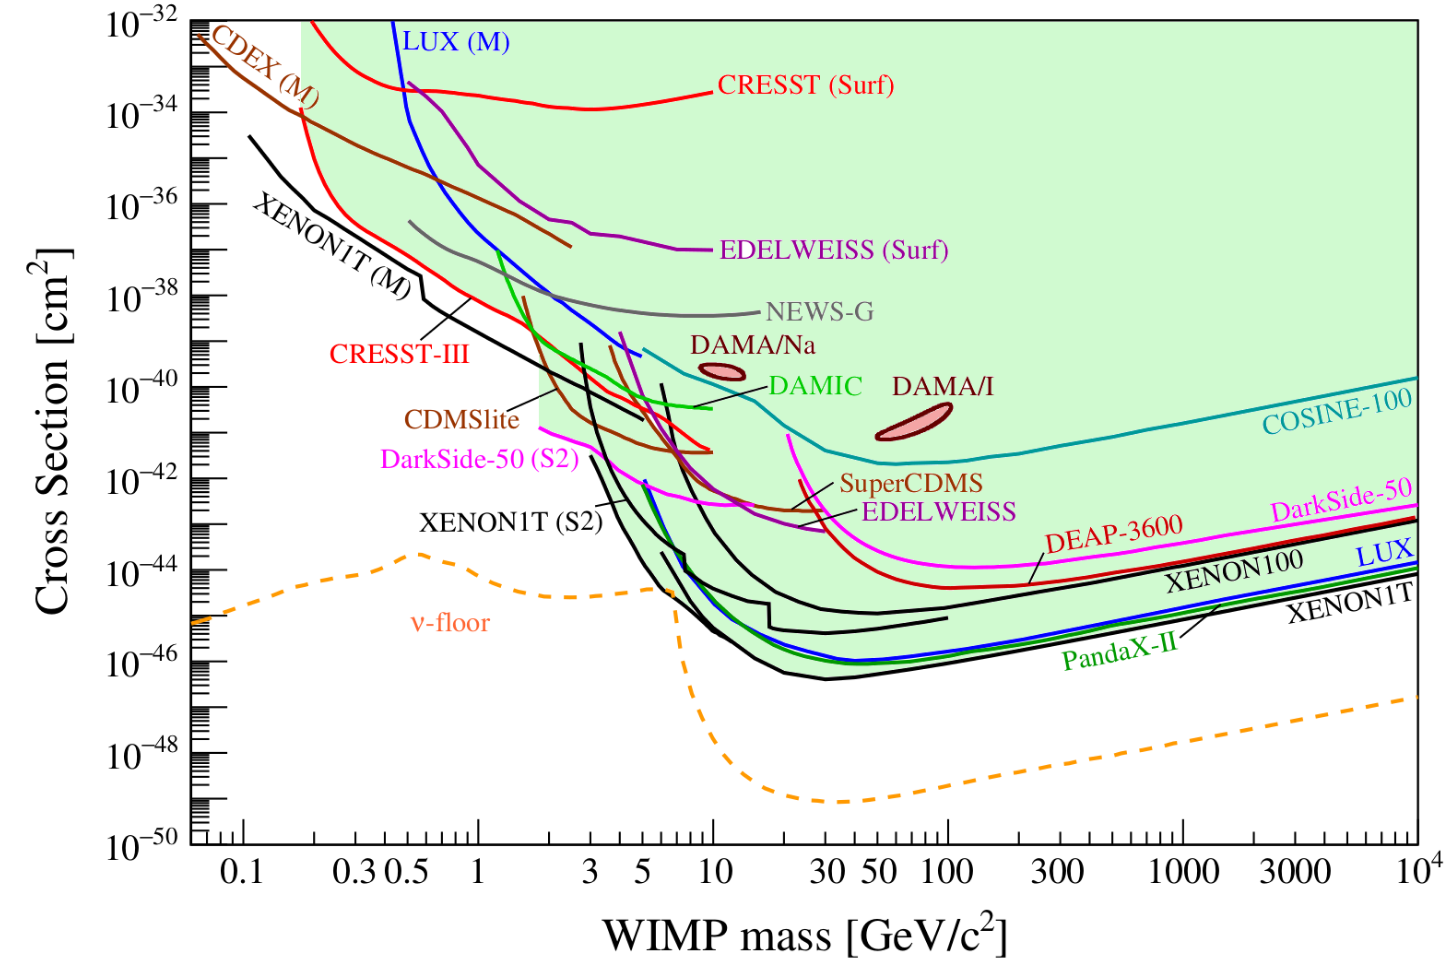
\includegraphics[width = 0.70 \textwidth]{dark-matter.png}
	\caption{Upper limit of WIMPs' interaction cross-section.}
	\label{dark-matter}
\end{figure}

\section{Energia oscura}

In cosmologia, l'energia oscura è una forma di energia proposta come causa dell'espansione accelerata dell'Universo. Questa energia oscura dovrebbe avere effetti solo su larga scala e si stima che abbia una densità di $ 6 \cdot 10^{-10} \,\text{J} \,\text{m}^{-3} \approx 7 \cdot 10^{-30} \,\text{g} \,\text{cm}^{-3} $, molto inferiore alla densità della materia barionica o della materia oscura: nonostante ciò, essendo distribuita uniformemente nell'Universo, essa è globalmente dominante.\\
Dopo aver formulato la teoria della Relatività Generale, Einstein si accorse che le soluzioni alle equazioni di campo prevedevano un Universo in espansione o in collasso, sebbene all'epoca si supponesse che l'Universo fosse statico: di conseguenza, introdusse un termine costante, denominato \textit{costante cosmologica} ed interpretata come la densità d'energia del vuoto, tale da cancellare gli effetti gravitazionali su larga scala.\\
Nel 1929, però, Hubble osservò invece che l'Universo sembra essere proprio in espansione: in particolare, dalle misure di redshift ricavò la \textit{legge di Hubble} per la velocità di allontanamento delle galassie in funzione della loro distanza dalla Terra:
\begin{equation}
	v = H_0 d
	\label{eq:11.4}
\end{equation}
dove $ H_0 \approx 70 \,\text{km}/\text{s} / \text{Mpc} $ è nota come costante di Hubble. Si vede dunque che più una galassia è lontana, più si allontana velocemente: questo è indice del fatto che l'espansione dell'Universo omogenea ed isotropa, in accordo col \textit{principio cosmologico}. Un'importante conseguenza dell'osservazione dell'espansione dell'Universo è che, ad un certo punto nel tempo, esso deve essere stato confinato in un singolo punto: questo viene detto Big Bang.\\
A seguito di questa scoperta, Einstein ritrattò sulla costante cosmologica, giudicata un errore. Negli anni 1960s, però, calcoli di QFT mostrarono che la densità di energia del vuoto non è zero, ma dovrebbe avere un valore estremamente grande e fisicamente insensato, a causa delle fluttuazioni quantistiche del vuoto: questo è tuttora noto come il problema della costante cosmologica.

\subsection{Modello di Friedmann}

L'Universo in espansione è modellato dalle equazioni di Friedmann, ricavate da quelle di Einstein, e le soluzioni sono di tre tipi:
\begin{enumerate}
	\item curvatura positiva ($ k = +1 $): l'Universo è un universo chiuso e ad un certo punto nel tempo inizierà a contrarsi, fino a ridursi di nuovo ad un punto;
	\item curvatura nulla ($ k = 0 $): l'Universo continuerà ad espandersi, ma l'espansione decellererà fino ad arrestarsi in un tempo infinito;
	\item curvatura negativa ($ k = -1 $): l'Universo continuerà ad espandersi, accellerando sempre di più.
\end{enumerate}
Il parametro di curvatura dell'Universo è legato al valore della densità media dell'Universo rispetto alla sua densità critica $ \rho_c \approx 9.47 \cdot 10^{-27} \,\text{kg} \, \text{m}^{-3} $: $ k = +1 $ se $ \rho > \rho_c $,  $ k = 0 $ se $ \rho = \rho_c $ e $ k = -1 $ se $ \rho < \rho_c $. È utile definire il \textit{parametro di densità} $ \Omega \defeq \rho / \rho_c $, che si può scrivere come:
\begin{equation}
	\Omega = \Omega_m + \Omega_r + \Omega_\Lambda
	\label{eq:11.5}
\end{equation}
$ \Omega_m $ è il contributo della materia barionica e di quella oscura, $ \Omega_r $ quello delle particelle relativistiche (fotoni e neutrini) e $ \Omega_\Lambda $ quello dovuto all'energia oscura. Le attuali stime danno $ \Omega = 1.02 \pm 0.02 $, dunque l'Universo dovrebbe essere prossimo alla densità critica.

\subsection{Evidenze sperimentali}

Le evidenze che suggeriscono l'esistenza dell'energia oscura sono indirette, ma sono tutte indipendenti tra loro:
\begin{enumerate}
	\item misure di wave patterns su larga scala della densità di massa nell'Universo;
	\item misure di distanza con supernovae di tipo Ia\footnote{sistemi binari con una consistente peak luminosity, dunque in grado di misurare con precisione le distanze tramite redshift (fino a $ 1000 \,\text{Mpc} $). Con questo metodo si è osservata l'espansione accellerata dell'Universo, valsa il Nobel nel 2011.};
	\item assenza di curvatura globale dalla CMB.
\end{enumerate}
In particolare, l'assenza di curvatura, ovverosia la globale piattezza dell'Universo, non può essere spiegata dalle sole materia barionica e oscura, le quali forniscono soltanto $ \approx 1/3 $ dell'energia totale richiesta. Per spiegare ciò e l'espansione accellerata dell'Universo, i cosmologi hanno proposto l'esistenza dell'energia oscura come legata alla costante cosmologica, in quanto omogenea ed isotropa nell'Universo.

\section{Evoluzione dell'Universo}

A seguito della scoperta dell'espansione dell'Universo da parte di Hubble si è capito che esso non è un sistema statico, ma ha un'evoluzione dettata dalle equazioni di Friedmann.\\
La temperatura media dell'Universo scala come $ T \sim a(t)^{-1} $, dove $ a(t) $ è il fattore di scala che ne determina la dimensione. Si possono dunque individuare dei periodi principali nella storia dell'Universo a partire dal Big Bang:
\begin{enumerate}
	\item $ t \sim 10^{-43} \,\text{s} $: \textit{Plank era}, di cui ancora non si hanno modelli fisici certi, data la predominanza della quantum gravity;
	\item $ t \sim 10^{-33} \,\text{s} $: \textit{Inflation}, durante la quale l'Universo subì un'espansione esponenziale a seguito di una vacuum phase transition;
	\item $ t \sim 10^{-32} \,\text{s} $: \textit{Grand Unification}, ovvero la separazione tra l'interazione forte e quella elettrodebole;
	\item $ t \sim 10^{-6} \,\text{s} $: \textit{Baryogenesis}, ovvero la transizione dai qarks liberi agli adroni;
	\item $ t \sim 1\,\text{ms} - 3\,\text{min} $: \textit{Nucleosynthesis}, con la formazione di $ \ch{D} $, $ \ch{He} $, $ \ch{Li} $ e $ \ch{Be} $;
	\item $ t \sim 10^5 \,\text{yr} $: \textit{radiation to matter dominance transition}, durante la quale si iniziarono a formare le prime strutture cosmiche;
	\item $ t \sim 380'000 \,\text{yr} $: \textit{Recombination}, in cui a seguito della neutralizzazione dell'idrogeno l'Universo divenne trasparente alla radiazione e venne emessa la CMBR;
	\item $ t \sim 0.3 - 1 \,\text{Gyr} $: \textit{Reionization}, con la formazione delle prime galassie.
\end{enumerate}
Empirical evidences of the thermal evolution of the Universe can be gathered by studying the CMBR, the various models for Nucleosynthesis, the matter-antimatter asymmetry (probing Baryogenesis) and the inflationary model.

\subsection{Planck era}

Con $ t \rightarrow 0 $ si $ a(t) \rightarrow 0 $, ovvero $ T \rightarrow \infty $, dunque approcciandosi al Big Bang diventano dominanti progressivamente tutte le interazioni fondamentali, rendendo sempre più difficile estrapolarne la fisica.\\
Fino a $ \sim 10^{-10} \,\text{s} $ si rimane nel regime testabile dagli accelleratori: in particolare, per $ T < 10^{15} \,\text{K} $ l'interazione elettromagnetica e quella debole sono separate, unendosi solo a $ T \sim 10^{28} \,\text{K} $, ed anche in questo regime è presente una teoria solida (quella Elettrodebole) che è stata ripetutamente testata sperimentalmente.\\
Spingendosi fino a $ \sim 10^{-35} \,\text{s} $, a $ T \sim 10^{29} \,\text{K} $ avviene la GUT phase transition, ovvero l'unificazione dell'interazione forte con quella elettrodebole: sebbene la teoria in questo caso sia relativamente solida, essa non è stata testata sperimentalmente.\\
Infine, nella Plank era, caratterizzata dal tempo di Plank $ t_\text{p} = \sqrt{c^{-5} \hbar G} \approx 5.39 \cdot 10^{-44} \,\text{s} $, si entra nell'ambito speculativo: si pensa che, data la dimensione dell'Universo $ l_\text{p} = c t_\text{p} \approx 1.62 \cdot 10^{-35} \,\text{m} $, avvenga un'unificazione di tutte le interazioni fondamentali, dunque per una descrizione teorica è necessaria una teoria di quantum gravity (es.: string theory, M-theory, ...).

\subsection{Inflation}

L'inflation model, formulato da Guth nel 1981, è supportato da evidenze empiriche come l'assenza di curvatura dell'Universo e l'uniformità della CMBR. In particolare, esso postula che a $ t \sim 10^{-34} \,\text{s} $ l'Universo si trovasse in una condizione di \textit{false vacuum}, ovvero in uno stato di energia maggiore di quella del ground state: essendo questo uno stato metastabile, esso decade nel ground state a seguito di una transizione di fase, la quale rilascia un'enorme quantità di energia latente. Proprio questa energia latente si pensa sia stata la causa dell'espansione esponenziale dell'Universo durante l'Inflation (un fattore di $ 10^{20} - 10^{30} $ in $ 10^{-36} - 10^{-32} \,\text{s} $).\\
L'inflation model risolve alcuni problemi della Big Bang cosmology:
\begin{enumerate}
	\item flatness problem: perché $ \Omega_0 \approx 1 $?
	\item horizon problem: perché la CMBR è così uniforme ($ \Delta T / T \sim 10^{-6} $)?
	\item monopole problem: perché non si osservano i numerosi monopoli magnetici che dovrebbero essere stati prodotti dal Big Bang?
\end{enumerate}
Inoltre, spiega naturalmente il power spectrum osservato per le density perturbations iniziali, oltre a predirne uno scale-invariant per il cosmic gravitational wave background.\\
In particolare, per quanto riguarda il flatness problem, a seguito dell'inflazione si ha localmente $ \Omega_0 \approx 1 $, ma per averlo anche a livello globale si dovrebbe avere, prima dell'Inflation, un Universo con $ \Omega $ praticamente uguale all'unità, ponendo un importante problema di fine-tuning (collegato all'anthropic principle).

\subsection{Quark-gluon plasma}

A parte per l'Inflation, è possibile predire con una certa accuratezza la temperatura dell'Universo andando indietro nel tempo: in particolare, la radiation temperature in un dato momento è legata alla massa caratteristica delle particelle presenti nell'Universo da $ mc^2 \sim kT $, dato che coppie particella-antiparticella vengono create e annichilite continuamente, dominando dunque il matter content dell'Universo. \\
Nei primi microsecondi dopo il Big Bang, l'Universo era dominato dalla radiazione: l'unica materia presente ($ \rho_m / \rho_r \sim 10^{-9} $) in questa epoch è il \textit{quark-gluon plasma}, un ensemble localizzato ed interagente di quark e gluoni in equilibrio termo-chimico (energia cinetica locale ed abbondanze relative). Una caratteristica importante del quark-gluon plasma è la presenza di free color charges, grazie ad una densità d'energia estremamente alta: a differenza della QCD classica, dunque, i gluoni non si comportano come force-carriers, ma sono deconfinati come i quarks. \\
È possibile produrre quark-gluon plasma anche nei collisori: in particolare, quando due nuclidi pesanti collidono ad alte energie, essi interagiscono tramite il color field, e nella zona d'interazione si viene a creare per brevissimo tempo uno stato di quark-gluon plasma, successivamente studiato tramite la rilevazione di prodotti di decadimento (coppie $ e^- e^+ $, $ \gamma $ e vari tipi di adroni). Al CERN questo tipo di collisioni sono studiate dall'esperimento ALICE.

\subsection{Bariogenesi}

Col raffreddamento dell'Universo nelle successive frazioni di secondo ($ \lesssim 10^{-4} \,\text{s} $, $ T \sim 10^{13} \,\text{K} $), i quarks nel quark-gluon plasma vengono confinati in barioni, sebbene l'energia media di collisione ($ \sim 1 \gev $) non permetta ancora la formazione di nuclidi. Inoltre, si noti che il Big Bang si pensa abbia prodotto un uguale quantitativo di materia ed antimateria: dato che oggi si osserva un quantitativo trascurabile di antimateria, questa è stata quasi completamente annichilita da un uguale quantità di materia (confermato dalla radiazione osservata nell'Universo attuale), dunque durante la bariogenesi ci deve essere stato un meccanismo per spiegare la \textit{baryonic asymmetry}, ovvero l'esistenza di una quantità maggiore di materia rispetto all'antimateria. Nel 1967 Sakharov ha proposto tre condizioni per spiegare questa asimmetria:
\begin{enumerate}
	\item scostamento dall'equilibrio termodinamico;
	\item violazione della conservazione del numero barionico;
	\item violazione della simmetria CP.
\end{enumerate}
Queste condizioni sono studiate da esperimenti al CERN: ALPHA, per la produzione di antiatomi, e LHCb, per lo studio della CP violation.

\subsection{Nucleosintesi}

A seguito della bariogenesi e fino a $ \sim 3 \,\text{min} $, le condizioni di energia e temperatura ($ T \sim 10^9 \,\text{K} $) permettono la formazione dei primi nuclidi leggeri ($ \ch{^2 H} $, $ \ch{^3 H} $, $ \ch{^3 He} $, $ \ch{^4 He} $, $ \ch{^7 Li} $ e $ \ch{^7 Be} $): si parla di \textit{Big Bang Nucleosynthesis} (BBN), mentre la successiva sintesi stellare dei nuclidi più pesanti è la \textit{Stellar Nucleosynthesis} (SN).\\
Il parametro che descrive gli effetti della BBN è il rapporto tra la densità numerica di barioni e quella di fotoni: $ n_b / n_\gamma \approx 6 \cdot 10^{-10} $. Da questo rapporto è possibile calcolare il rate di reazione tra nucleoni (Fig. \ref{bbn}), oltre che le abbondanze relative delle varie specie chimiche: $ \sim 75\% $ di idrogeno, $ \sim 25\% $ di elio e tracce di litio e berillio. Le abbondanze così calcolate sono consistenti con quelle osservate, e ciò è considerato una strong evidence della teoria del Big Bang.\\
Durante la BBN si instaura un equilibrio dinamico tra materia e radiazione tramite reazioni di fotodissociazione: col calare della temperatura, però, queste reazioni cessano, e con $ T \lesssim 3 \cdot 10^8 \,\text{K} $ cessa anche la fusione dei nuclei leggeri: questo è il termine della BBN, oltre il quale le abbondanze relative delle varie specie nucleari rimangono approssimativamente invariate.\\
Con i dati estratti dalla CMBR (vedere Sec. \ref{sec-cmbr}) è possibile predirre le relative mass abundances delle specie nucleari prodotte dalla BBN e compararle con quelle predette dalla teoria della BBN e con quell osservate astronomicamente nei cosiddetti \textit{Schramm plots}: nel caso del $ \ch{^2 H} $ e del $ \ch{^4 He} $ c'è un accordo tra la previsione teorica e le osservazioni empiriche, mentre per quanto riguarda il $ \ch{^7 Li} $ si osserva una relative mass abundance minore di un fattore di 3 rispetto alla previsione del modello BBN; quest'ultimo è noto come \textit{cosmological} $ \ch{^7 Li} $ \textit{problem}.\\
Gli elementi più pesanti vengono prodotti dalla SN tramite reazioni di fusione (capace di produrre fino al $ \ch{^{56} Fe} $: queste reazioni sono studiate da esperimenti sotterranei come LUNA@LNGS, in quanto la cross-section di fusione nucleare ad energie d'interesse astrofisico è estremamente bassa (Coulomb barrier), dunque, non avendo a disposizione l'enorme quantità di combustibile presente nelle stelle, si hanno rate nell'ordine di $ 1 \text{evento} / \text{mese} - 1 \text{evento} / \text{giorno} $ ed è necessario minimizzare il rumore. È possibile anche la produzione di nuclei oltre il $ \ch{^{56} Fe} $ con reazioni di fissione o r-process (vedere Sec. \ref{sec-stell-av}): lo studio di queste reazione richiede tecniche sperimentali sofisticate, in quanto sono necessari fasci instabili di ioni radioattivi; si pensa che lo studio dell'r-process, basato sulla competizione tra cattura neutronica e decadimento $ \beta^- $, possa portare al popolamento della Terra Incognita adiacente alla neutron dripline (Fig. \ref{drip-lines}), essendo esso influenzato dalla deformazione dei nuclidi coinvolti: più un nucleo è deformato, più alta sarà la sua vita media rispetto al decadimento $ \beta^- $ e più bassa la sua neutron emission probability.

\begin{figure}[b]
	\centering
	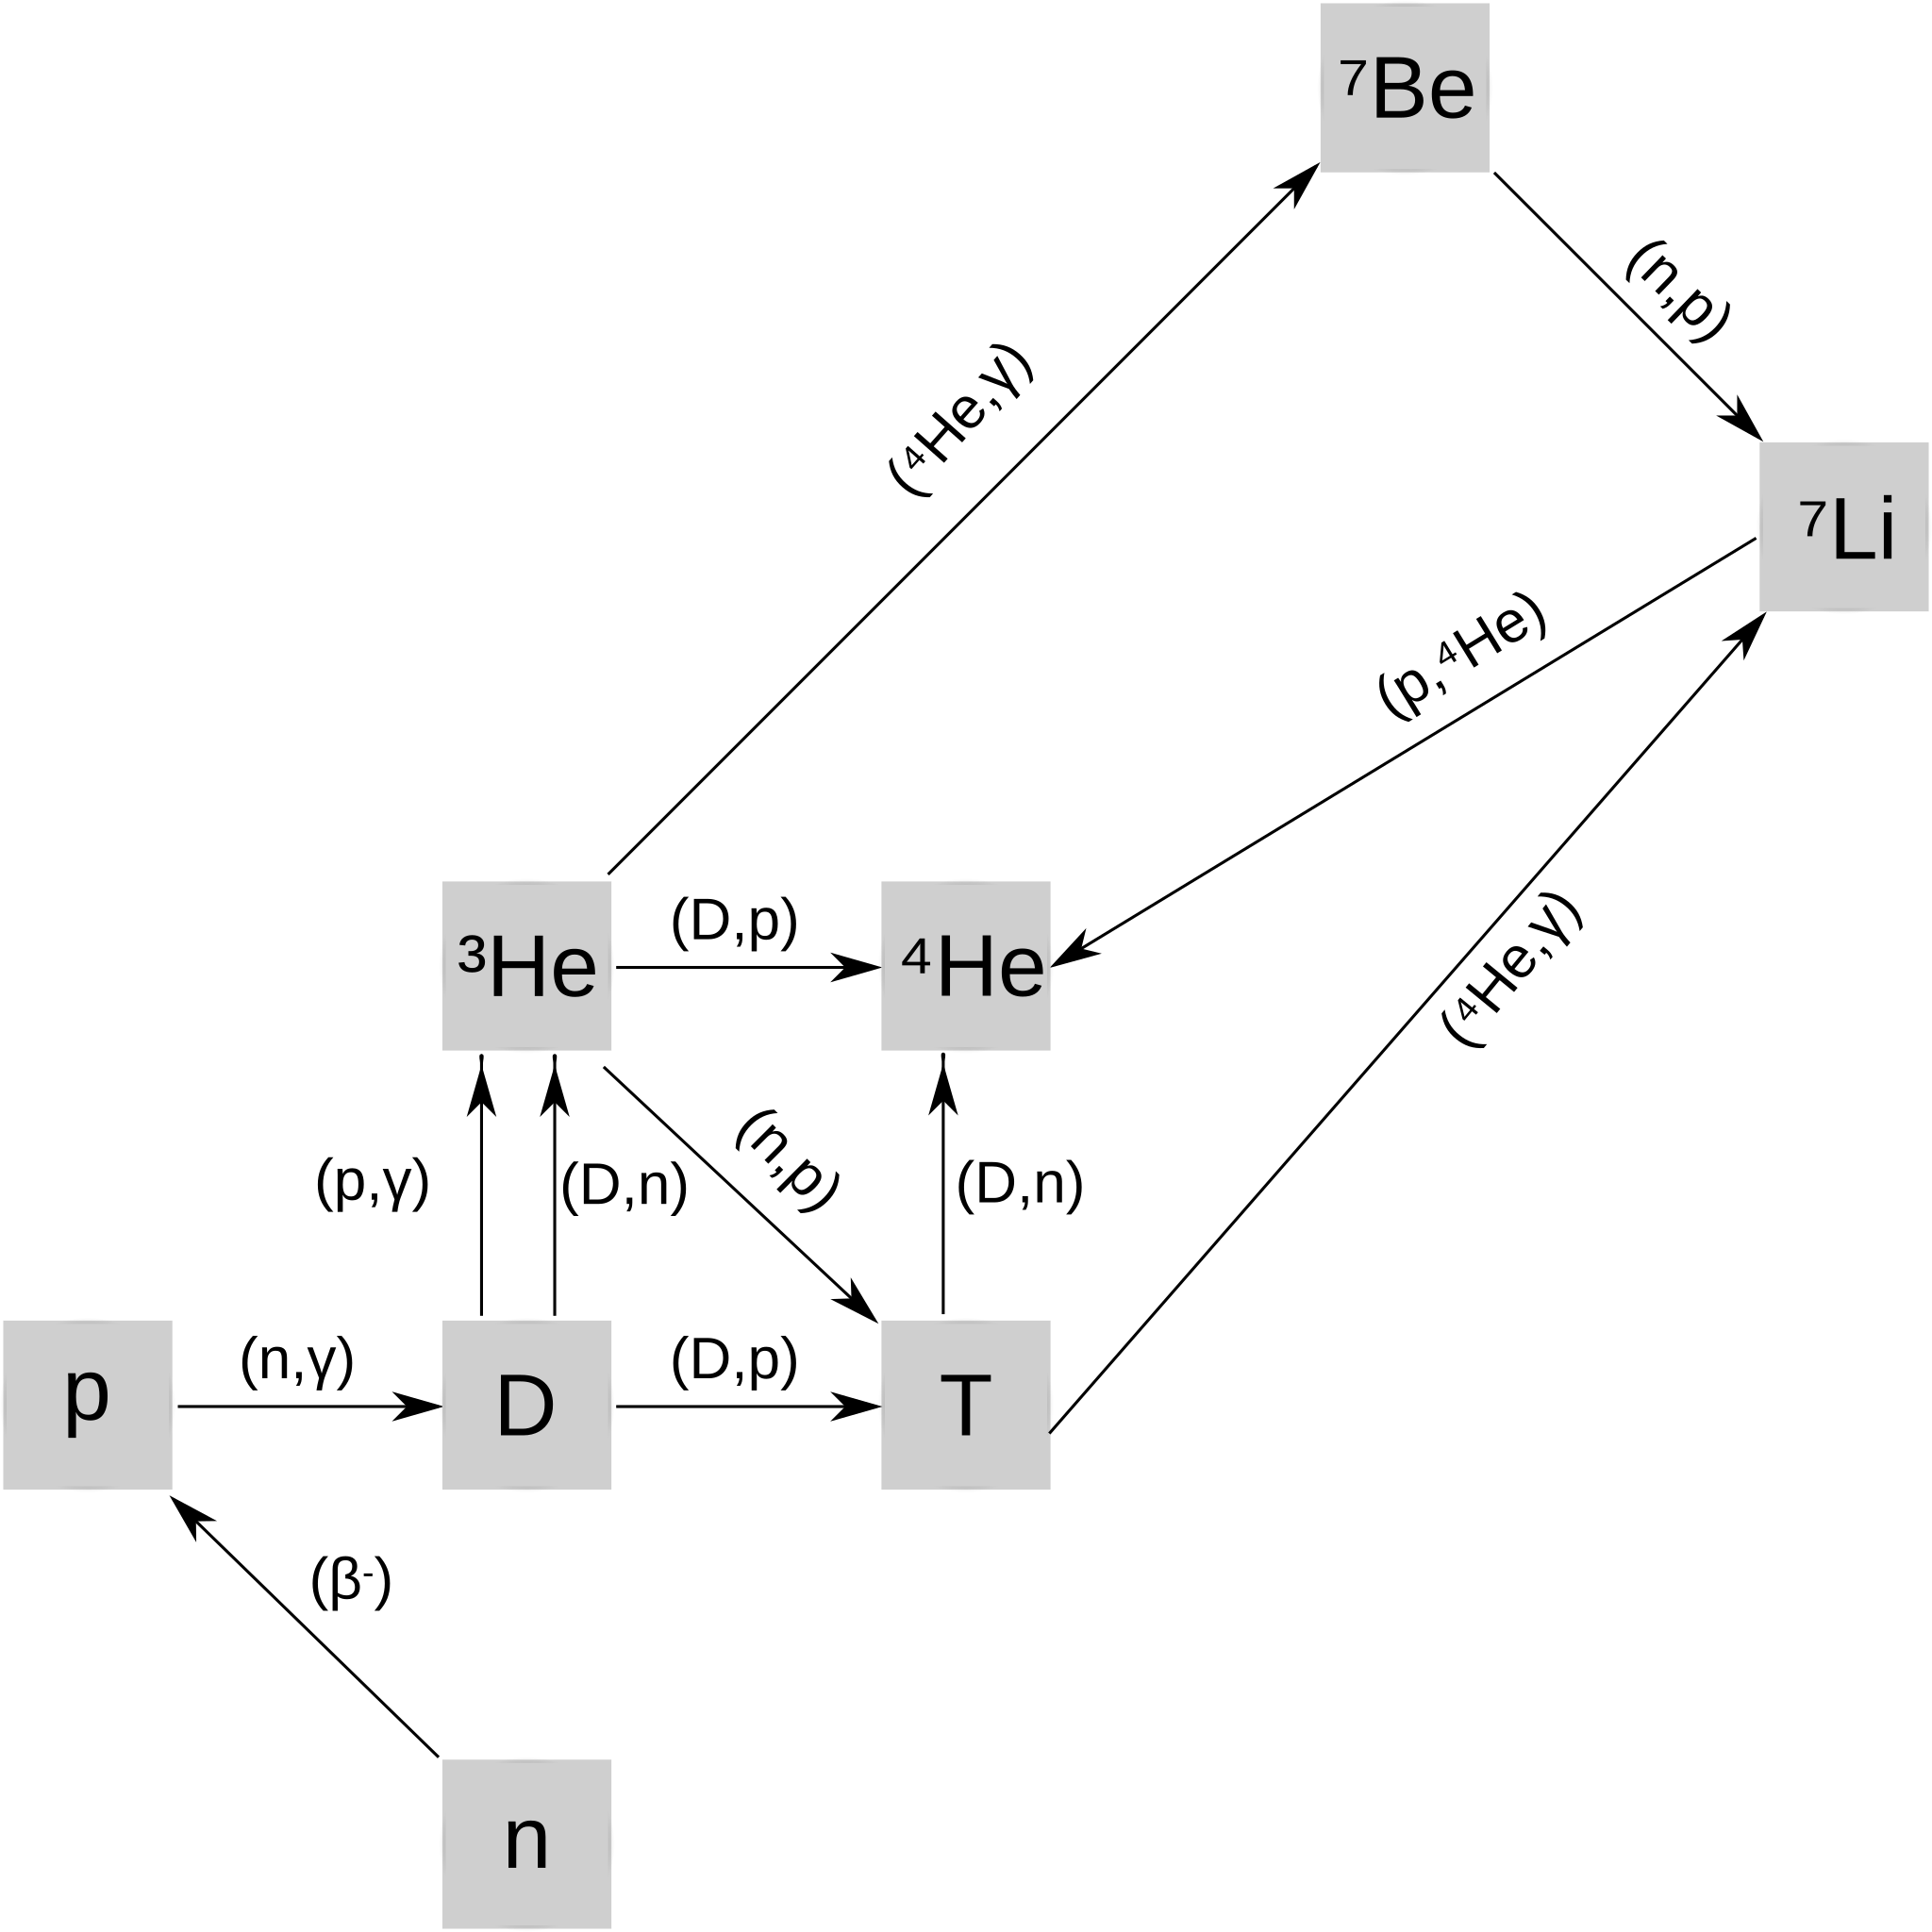
\includegraphics[width = 0.60 \textwidth]{bbn.png}
	\caption{Main reaction chain of BBN.}
	\label{bbn}
\end{figure}

\subsection{Cosmic Microwave Background}
\label{sec-cmbr}

A seguito dell'inflation, l'Universo era opaco alla radiazione, in quanto il libero cammino medio dei fotoni era estremamente corto, data l'altissima probabilità di interazione con le particelle di materia libere. Dopo la nucleosintesi e centinaia di migliaia di anni di raffreddamento, però, col confinamento della materia negli atomi neutri, l'Universo diventa trasparente: questa è l'era della \textit{Recombination}, in cui i fotoni hanno libero cammino medio praticamente infinito e possono propagarsi fino all'epoca odierna sotto forma di \textit{Cosmic Microwave Background Radiation} (CMBR).\\
L'esistenza della CMBR è stata predetta da Gamow, Alpher ed Herman nel 1949 sulla base del modello a Big Bang: uno stato iniziale caldo e ionizzato deve produrre radiazione termica, la quale, a seguito della ricombinazione, deve essere libera di propagarsi nello spaziotempo. In particolare, sull base della relazione $ T(t) \sim T_0 / a(t) $, essi stimarono che al giorno d'oggi la CMBR dovrebbe avere $ T \sim 5 \,\text{K} $ (osservata a $ T \approx 2.7 \,\text{K} $).\\
L'osservazione della CMBR fu fatta nel 1965 da Penzias e Wilson: essi osservarono un fondo nelle onde radio circa 100 volte più intenso di quello previsto, omogeneo nella distribuzione angolare e nel tempo. Con tecniche di elaborazione sofisticate si può estrarre dal brackground omogeneo l'originale CMBR: bisogna considerare la presenza di due lobi di redshift e blueshift, dovuti all'effetto Doppler determinato dal moto del sistema solare rispetto al background, e la presenza della radiazione a microonde prodotta dalla Via Lattea; a seguito di queste sottrazioni (ed aumentando il contrasto) si ottiene la Fig. \ref{cmbr}.
Le misure della CMBR confermano la sua estrema uniformità ($ \Delta T / T \sim 10^{-6} $): ciò viene spiegato dal fatto che l'Universo è il risultato dell'inflazione di un volume estremamente piccolo ed a condizioni iniziali sostanzialmente identiche. Inoltre, interpolando l'andamento delle CMB fluctuations con delle armoniche sferiche, è possibile estrarre il cosiddetto \textit{anisotropy power spectrum}: la posizione dei picchi di questo spettro dipende sensibilmente dalla curvatura spaziale dell'Universo, dunque dal suo studio è possibile porre dei constraints alle proprietà della dark energy.

\begin{figure}
	\centering
	\includegraphics[width = 0.70 \textwidth]{cmbr.png}
	\caption{CMBR from WMAP.}
	\label{cmbr}
\end{figure}










